\documentclass[11pt]{scrartcl}
\newcommand*\student[1]{\newcommand{\thestudent}{{#1}}}
\newcommand*\course[1]{\newcommand{\thecourse}{{#1}}}
\newcommand*\courseshort[1]{\newcommand{\thecourseshort}{{#1}}}
\newcommand*\assnumber[1]{\newcommand{\theassnumber}{{#1}}}

\student{Stefano Taillefert}
\course{Machine Learning}
\courseshort{ML}
\assnumber{2}

%----------------------------------------------------------------------------------------
%	PACKAGES AND OTHER DOCUMENT CONFIGURATIONS
%----------------------------------------------------------------------------------------

\usepackage[utf8]{inputenc} % Required for inputting international characters
\usepackage[T1]{fontenc} % Use 8-bit encoding
\usepackage[sc]{mathpazo}
\usepackage{caption, subcaption}
\usepackage[hidelinks]{hyperref}
\usepackage{inconsolata}

\usepackage[english]{babel} % English language hyphenation
\usepackage{amssymb}
\usepackage{amsmath}% Math packages
\usepackage{listings} % Code listings, with syntax highlighting
\usepackage{graphicx} % Required for inserting images
\usepackage{float}

%----------------------------------------------------------------------------------------
%	DOCUMENT MARGINS
%----------------------------------------------------------------------------------------

\usepackage{geometry} % For page dimensions and margins
\geometry{
	paper=a4paper, 
	top=2.5cm, % Top margin
	bottom=3cm, % Bottom margin
	left=3cm, % Left margin
	right=3cm, % Right margin
}
\setlength\parindent{0pt}

%----------------------------------------------------------------------------------------
%	SECTION TITLES
%----------------------------------------------------------------------------------------

\usepackage{sectsty}
\sectionfont{\vspace{6pt}\centering\normalfont\scshape}
\subsectionfont{\normalfont\bfseries} % \subsection{} styling
\subsubsectionfont{\normalfont\itshape} % \subsubsection{} styling
\paragraphfont{\normalfont\scshape} % \paragraph{} styling

%----------------------------------------------------------------------------------------
%	HEADERS AND FOOTERS
%----------------------------------------------------------------------------------------

\usepackage{scrlayer-scrpage}
\ofoot*{\pagemark} % Right footer
\ifoot*{\thestudent} % Left footer
\cfoot*{\thecourseshort \ assignment \theassnumber} % Centre footer

%----------------------------------------------------------------------------------------
%	TITLE SECTION
%----------------------------------------------------------------------------------------

\title{	
	\normalfont\normalsize
	\textsc{\thecourse\\%
	Università della Svizzera italiana}\\
	\vspace{25pt}
	\rule{\linewidth}{0.5pt}\\
	\vspace{20pt}
	{\huge Assignment \theassnumber}\\
	\vspace{12pt}
	\rule{\linewidth}{0.5pt}\\
	\vspace{12pt}
}

\author{\LARGE \thestudent}

\date{\normalsize\today}

\begin{document}

\maketitle

%----------------------------------------------------------------------------------------
%%	PROBLEMS - EDIT HERE
%----------------------------------------------------------------------------------------

\section*{Intro}

	The submission archive includes all the necessary code, but the model files must be retrieved from:\\

	\url{https://github.com/Steeven9/ML-Assignment-2}\\

	The repo will be made public shortly after the deadline to avoid surprises; also since it's versioned you can check that the models were not updated after the deadline.\\

	To run the models, simply \texttt{cd} into \texttt{deliverable/} and run \texttt{run\_task1.py} or \texttt{run\_task2.py}. Make sure to have the \texttt{custom\_utils.py} file in the same directory!\\

	To compile and train the models, run \texttt{create\_models.py [task\_number]} from the \texttt{src} folder. Without arguments, both tasks will be executed. The \texttt{custom\_utils.py} file is required here as well (yes, two copies are already included in both folders for convenience).\\

	In both cases the script will automatically download the necessary datasets, so everything should work out of the box on first try. Hopefully.


\newpage
\section*{Problem 1}

	1. - 4. The model is in the file \texttt{deliverable/nn\_task1.h5}, while the code used to 
	generate it is in the first section of \texttt{src/create\_models.py}.\\
	For this task I ran all the code on my Mac without encountering particular problems.\\
	
	5. Here's the plot I obtained:

	\begin{figure}[H]
		\centering
		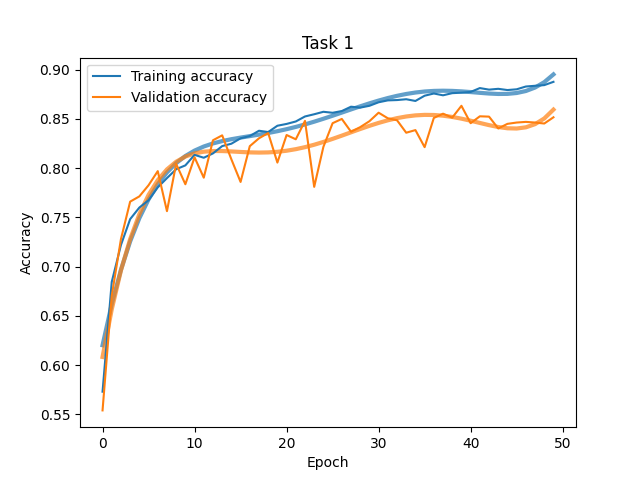
\includegraphics[width=\textwidth]{src/plot_task1.png}
		\caption{The plot for task 1}
		\label{fig:plot_T1}
	\end{figure}

	6. - 7. The results from the various models are summarized in the table below:\\
	
	\begin{table}[H]
		\centering
		\begin{tabular}{cccc}
			Model & Test loss & Accuracy & MSE\\
			\hline
			8 neurons - 0.003 LR & 0.3513 & 0.8653 & 0.0669\\
			16 neurons - 0.01 LR & 0.4168 & 0.8337 & 0.0790\\
			64 neurons - 0.01 LR & 0.4315 & 0.8297 & 0.0812\\
			16 neurons - 0.0001 LR & 0.3693 & 0.8540 & 0.0704\\
			64 neurons - 0.0001 LR & 0.3956 & 0.8410 & 0.0757
		\end{tabular}
	\end{table}

	All five models have been trained and evaluated in sequence on the same dataset.\\
	
	\newpage
	Futhermore, a statistical analysis has been conducted, and below is the output:\\

	\begin{figure}[H]
		\centering
		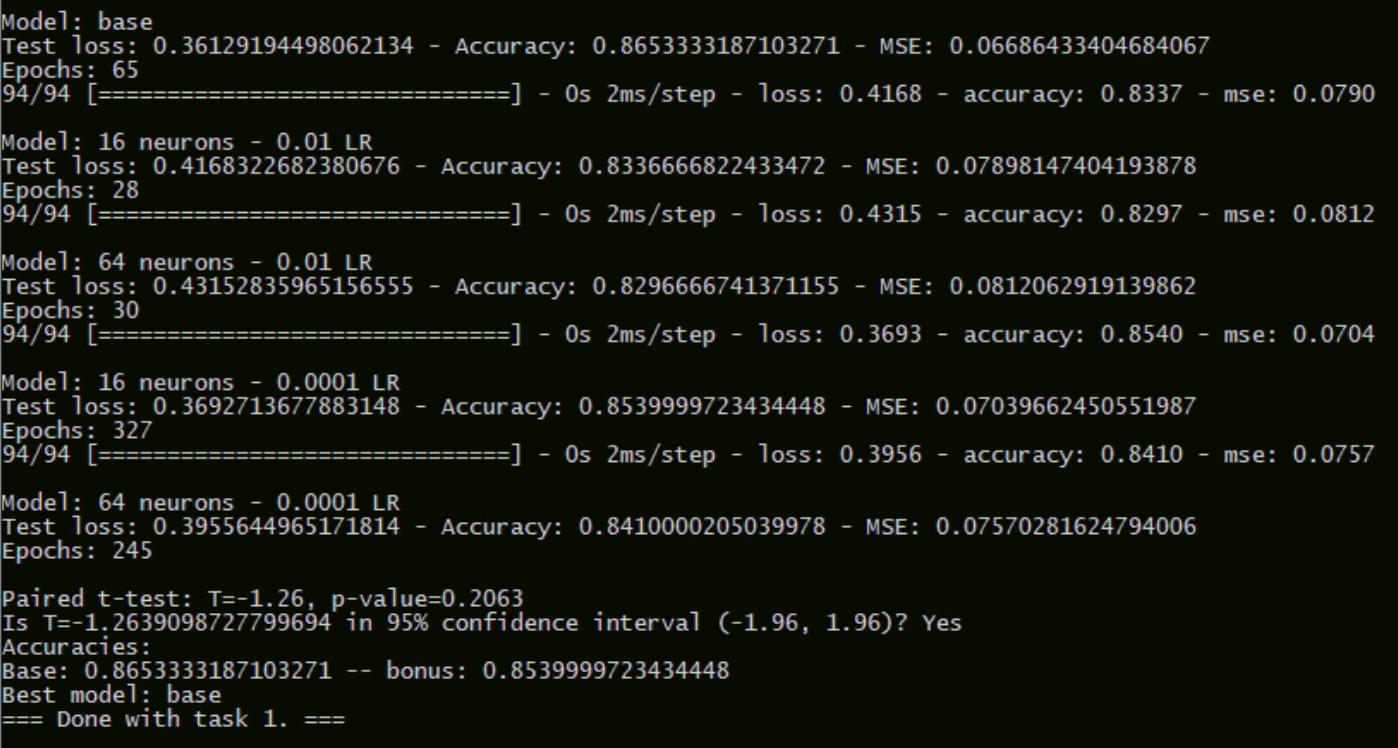
\includegraphics[width=\textwidth]{src/result.png}
		\caption{The result of the statistical analysis}
		\label{fig:result}
	\end{figure}

	As we can see, the paired Student's t-test indicates that our initial hypothesis,
	which is that the two models are equivalent, is accepted: the T value is in the
	95\% confidence interval, so this means that the compared samples are very similar. 
	The p-value is also relatively big (> 0.005), so this further confirms the correlation.
	Therefore we pick the model with the highest accuracy between the two, since they
	are statistically very equivalent.\\

	According to our data, the best model is the base one (8 neurons - 0.003 learning rate).


\newpage
\section*{Problem 2}

	1. - 3. See the following sections for the details of the behavior of the two models. In both cases the hidden layer I added is a dense one with 128 neurons and ReLu activation function, while the output layer has three neurons since we have three classes (rock, paper, scissors).\\

	4. For this task I tried to use my gaming rig at home (Intel i5-9600K, 16GB DDR4@3200, RTX 2060) instead of Colab. I spent a whole day struggling with CUDA and Python on Windows 10 (ugh) and after some fiddling I managed to make it work. The first part, without data augmentation, worked fine, but for the second part I ran out of VRAM after the first epoch. That was a bit underwhelming to say the least.\\
	I included both the result from Colab and my machine for the first part, while the second one has been run only on the cloud.\\

	I am unaware if it's a hard limitation or if I could tune the model to get around it (maybe less neurons for the hidden layer?); despite the fact that I would've loved to run everything locally, I didn't have much time left to investigate further. Here's the error I got:\\
	\texttt{W tensorflow/core/common\_runtime/bfc\_allocator.cc:456] Allocator (GPU\_0\_bfc) ran
	out of memory trying to allocate 3.59GiB (rounded to 3853516800)requested by op
	sequential\_6/vgg16/block1\_conv1/Relu}


	\subsection*{Without augmentation}

		\begin{figure}[H]
			\centering
			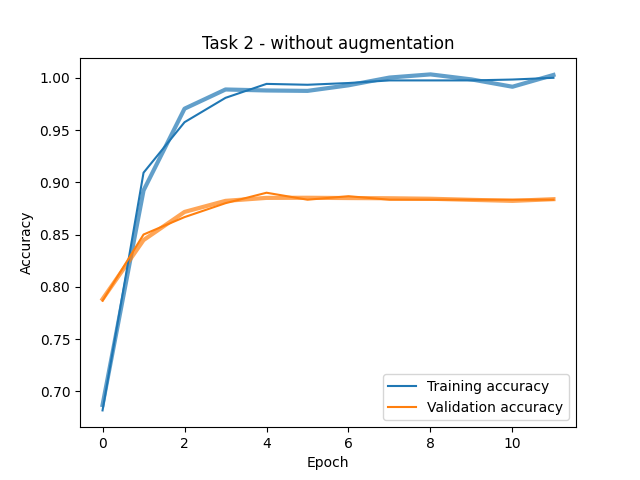
\includegraphics[width=\textwidth]{src/plot_task2_no_augmentation.png}
			\caption{The plot for task 2 without data augmentation}
			\label{fig:plot_T2_1}
		\end{figure}

		The results from the model without augmentation are:\\
		
		Test loss: 0.2259 - Accuracy: 0.9366 - MSE: 0.0319 (my pc)\\
		Test loss: 0.3201 - Accuracy: 0.9100 - MSE: 0.0464 (Colab)\\

		The model is in the files \texttt{deliverable/nn\_task2\_no\_augmentation.h5} and\\ 
		\texttt{deliverable/nn\_task2\_no\_augmentation.pkl} (you can choose which one to run, they should be the same), while the code used to generate 
		it is in the second section of \texttt{src/create\_models.py}


	\subsection*{With augmentation}

		\begin{figure}[H]
			\centering
			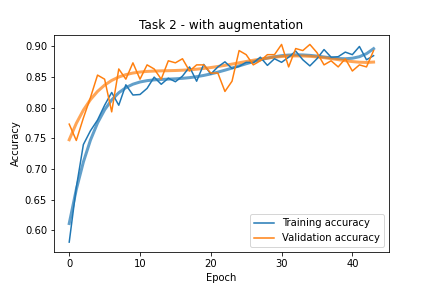
\includegraphics[width=\textwidth]{src/plot_task2_augmentation.png}
			\caption{The plot for task 2 with data  augmentation}
			\label{fig:plot_T2_2}
		\end{figure}

		The results from the model with augmentation are:\\
		
		Test loss: 0.2214 - Accuracy: 0.9133 - MSE: 0.0421 (Colab)\\

		The model is in the files \texttt{deliverable/nn\_task2\_augmentation.h5} and\\ 
		\texttt{deliverable/nn\_task2\_augmentation.pkl} (you can choose which one to run, they should be the same), while the code used to generate 
		it is in the second section of \texttt{src/create\_models.py}\\


	\newpage
	\subsection*{Conclusion}

		Based on the experimental results, using data augmentation didn't improve much our model; instead we actually obtained worse scores than without it. Here's a summary of the values:

		\begin{table}[H]
			\centering
			\begin{tabular}{cccc}
				Model & Test loss & Accuracy & MSE\\
				\hline
				No augmentation (local) & 0.2259 & 0.9366 & 0.0319\\
				No augmentation (Colab) & 0.3201 & 0.9100 & 0.0464\\
				With augmentation (Colab) & 0.2214 & 0.9133 & 0.0421
			\end{tabular}
		\end{table}

		As we can see, the three values are not very far from eachother. Test loss and accuracy decreased - which are respectively a good and bad thing - while MSE went up, which is definitely not good. On the other hand, those are very little varainces and one could argue that an accuracy of 0.9366 is already very good, so there is not much room for improvement anyway.\\

		The interesting part is that I obtained better results running the code on my machine rather than on Google's platform, despite having the exact same code, data and seeds for tensorflow and numpy (just in case).


\end{document}
